% Options for packages loaded elsewhere
\PassOptionsToPackage{unicode}{hyperref}
\PassOptionsToPackage{hyphens}{url}
%
\documentclass[
]{article}
\usepackage{lmodern}
\usepackage{amssymb,amsmath}
\usepackage{ifxetex,ifluatex}
\ifnum 0\ifxetex 1\fi\ifluatex 1\fi=0 % if pdftex
  \usepackage[T1]{fontenc}
  \usepackage[utf8]{inputenc}
  \usepackage{textcomp} % provide euro and other symbols
\else % if luatex or xetex
  \usepackage{unicode-math}
  \defaultfontfeatures{Scale=MatchLowercase}
  \defaultfontfeatures[\rmfamily]{Ligatures=TeX,Scale=1}
\fi
% Use upquote if available, for straight quotes in verbatim environments
\IfFileExists{upquote.sty}{\usepackage{upquote}}{}
\IfFileExists{microtype.sty}{% use microtype if available
  \usepackage[]{microtype}
  \UseMicrotypeSet[protrusion]{basicmath} % disable protrusion for tt fonts
}{}
\makeatletter
\@ifundefined{KOMAClassName}{% if non-KOMA class
  \IfFileExists{parskip.sty}{%
    \usepackage{parskip}
  }{% else
    \setlength{\parindent}{0pt}
    \setlength{\parskip}{6pt plus 2pt minus 1pt}}
}{% if KOMA class
  \KOMAoptions{parskip=half}}
\makeatother
\usepackage{xcolor}
\IfFileExists{xurl.sty}{\usepackage{xurl}}{} % add URL line breaks if available
\IfFileExists{bookmark.sty}{\usepackage{bookmark}}{\usepackage{hyperref}}
\hypersetup{
  pdftitle={Using a Pareto distribution to model the relationship of COVID19 test positivity and true case numbers},
  pdfauthor={Michael T Bretscher},
  hidelinks,
  pdfcreator={LaTeX via pandoc}}
\urlstyle{same} % disable monospaced font for URLs
\usepackage[margin=1in]{geometry}
\usepackage{color}
\usepackage{fancyvrb}
\newcommand{\VerbBar}{|}
\newcommand{\VERB}{\Verb[commandchars=\\\{\}]}
\DefineVerbatimEnvironment{Highlighting}{Verbatim}{commandchars=\\\{\}}
% Add ',fontsize=\small' for more characters per line
\usepackage{framed}
\definecolor{shadecolor}{RGB}{248,248,248}
\newenvironment{Shaded}{\begin{snugshade}}{\end{snugshade}}
\newcommand{\AlertTok}[1]{\textcolor[rgb]{0.94,0.16,0.16}{#1}}
\newcommand{\AnnotationTok}[1]{\textcolor[rgb]{0.56,0.35,0.01}{\textbf{\textit{#1}}}}
\newcommand{\AttributeTok}[1]{\textcolor[rgb]{0.77,0.63,0.00}{#1}}
\newcommand{\BaseNTok}[1]{\textcolor[rgb]{0.00,0.00,0.81}{#1}}
\newcommand{\BuiltInTok}[1]{#1}
\newcommand{\CharTok}[1]{\textcolor[rgb]{0.31,0.60,0.02}{#1}}
\newcommand{\CommentTok}[1]{\textcolor[rgb]{0.56,0.35,0.01}{\textit{#1}}}
\newcommand{\CommentVarTok}[1]{\textcolor[rgb]{0.56,0.35,0.01}{\textbf{\textit{#1}}}}
\newcommand{\ConstantTok}[1]{\textcolor[rgb]{0.00,0.00,0.00}{#1}}
\newcommand{\ControlFlowTok}[1]{\textcolor[rgb]{0.13,0.29,0.53}{\textbf{#1}}}
\newcommand{\DataTypeTok}[1]{\textcolor[rgb]{0.13,0.29,0.53}{#1}}
\newcommand{\DecValTok}[1]{\textcolor[rgb]{0.00,0.00,0.81}{#1}}
\newcommand{\DocumentationTok}[1]{\textcolor[rgb]{0.56,0.35,0.01}{\textbf{\textit{#1}}}}
\newcommand{\ErrorTok}[1]{\textcolor[rgb]{0.64,0.00,0.00}{\textbf{#1}}}
\newcommand{\ExtensionTok}[1]{#1}
\newcommand{\FloatTok}[1]{\textcolor[rgb]{0.00,0.00,0.81}{#1}}
\newcommand{\FunctionTok}[1]{\textcolor[rgb]{0.00,0.00,0.00}{#1}}
\newcommand{\ImportTok}[1]{#1}
\newcommand{\InformationTok}[1]{\textcolor[rgb]{0.56,0.35,0.01}{\textbf{\textit{#1}}}}
\newcommand{\KeywordTok}[1]{\textcolor[rgb]{0.13,0.29,0.53}{\textbf{#1}}}
\newcommand{\NormalTok}[1]{#1}
\newcommand{\OperatorTok}[1]{\textcolor[rgb]{0.81,0.36,0.00}{\textbf{#1}}}
\newcommand{\OtherTok}[1]{\textcolor[rgb]{0.56,0.35,0.01}{#1}}
\newcommand{\PreprocessorTok}[1]{\textcolor[rgb]{0.56,0.35,0.01}{\textit{#1}}}
\newcommand{\RegionMarkerTok}[1]{#1}
\newcommand{\SpecialCharTok}[1]{\textcolor[rgb]{0.00,0.00,0.00}{#1}}
\newcommand{\SpecialStringTok}[1]{\textcolor[rgb]{0.31,0.60,0.02}{#1}}
\newcommand{\StringTok}[1]{\textcolor[rgb]{0.31,0.60,0.02}{#1}}
\newcommand{\VariableTok}[1]{\textcolor[rgb]{0.00,0.00,0.00}{#1}}
\newcommand{\VerbatimStringTok}[1]{\textcolor[rgb]{0.31,0.60,0.02}{#1}}
\newcommand{\WarningTok}[1]{\textcolor[rgb]{0.56,0.35,0.01}{\textbf{\textit{#1}}}}
\usepackage{longtable,booktabs}
% Correct order of tables after \paragraph or \subparagraph
\usepackage{etoolbox}
\makeatletter
\patchcmd\longtable{\par}{\if@noskipsec\mbox{}\fi\par}{}{}
\makeatother
% Allow footnotes in longtable head/foot
\IfFileExists{footnotehyper.sty}{\usepackage{footnotehyper}}{\usepackage{footnote}}
\makesavenoteenv{longtable}
\usepackage{graphicx}
\makeatletter
\def\maxwidth{\ifdim\Gin@nat@width>\linewidth\linewidth\else\Gin@nat@width\fi}
\def\maxheight{\ifdim\Gin@nat@height>\textheight\textheight\else\Gin@nat@height\fi}
\makeatother
% Scale images if necessary, so that they will not overflow the page
% margins by default, and it is still possible to overwrite the defaults
% using explicit options in \includegraphics[width, height, ...]{}
\setkeys{Gin}{width=\maxwidth,height=\maxheight,keepaspectratio}
% Set default figure placement to htbp
\makeatletter
\def\fps@figure{htbp}
\makeatother
\setlength{\emergencystretch}{3em} % prevent overfull lines
\providecommand{\tightlist}{%
  \setlength{\itemsep}{0pt}\setlength{\parskip}{0pt}}
\setcounter{secnumdepth}{-\maxdimen} % remove section numbering
\usepackage{xfrac}
\usepackage{float}
\usepackage{booktabs}
\usepackage{longtable}
\usepackage{array}
\usepackage{multirow}
\usepackage{wrapfig}
\usepackage{colortbl}
\usepackage{pdflscape}
\usepackage{tabu}
\usepackage{threeparttable}
\usepackage{threeparttablex}
\usepackage[normalem]{ulem}
\usepackage{makecell}

\title{Using a Pareto distribution to model the relationship of COVID19
test positivity and true case numbers}
\author{Michael T Bretscher}
\date{Mon Dec 7 10:14:20 2020}

\begin{document}
\maketitle

\hypertarget{background}{%
\section{Background}\label{background}}

\begin{itemize}
\item
  During the course of the covid\_19 pandemic, the proportion of
  positive tests was highlighted as an important indicator of case
  underreporting.
\item
  Very low values of test positivity suggest a small proportion of
  undetected cases.
\item
  Conversely, case numbers are less reliable as test positivity
  increases, with more cases going undetected.
\item
  Test positivity, and how it changes with the number of tests conducted
  per population, is a consequence of how individuals are chosen for
  testing.
\item
  With random testing, test positivity should be equal to infection
  prevalence in the population, independently of testing coverage (no.
  of tests per population).
\item
  However, if testing is targeted, with high-risk individuals tested
  first, a monotonic decrease in test positivity with testing coverage
  is expected.
\item
  Individuals at high risk of prevalent infection may be identified in
  various ways, such as presence of various symptoms, connection to
  other cases, location, etc.
\item
  While the mentioned qualitative insights on test positivity are widely
  applied to interpret covid19 testing data, there has to my knowledge
  not been a simple formula available that directly relates test
  postivity and the amount of case underreporting in a quantitative way.
\item
  Such a formula could be used to inform policy by 1) providing
  estimates of true case numbers when test positivity is high, 2)
  predict the impact of ramping up testing on the proportion of detected
  cases (and hence on transmission reduction through case finding), and
  3) to describe and compare testing strategies across geographic areas
  through comparison of formula parameters estimated from area-specific
  data.
\end{itemize}

\hypertarget{objectives}{%
\section{Objectives}\label{objectives}}

\begin{itemize}
\item
  To derive a quantitative modeling framework relating test positivity,
  testing coverage, and case underreporting
\item
  To fit the model to data, in order to estimate unknown model
  parameters and assess model adequacy.
\item
  To demonstrate the application of this framework to answer questions
  on true case numbers and on the expected transmission-reducing benefit
  of additional testing.
\end{itemize}

\newpage

\hypertarget{the-pareto-distribution}{%
\section{The Pareto distribution}\label{the-pareto-distribution}}

The proportion of detected cases as function of the testing coverage
(tests conducted per true case) is assumed to follow the CDF of a Pareto
distribution.

\textbf{Pareto Type I distribution (Source: Wikipedia):}

\begin{center}
\begin{figure}[H]
  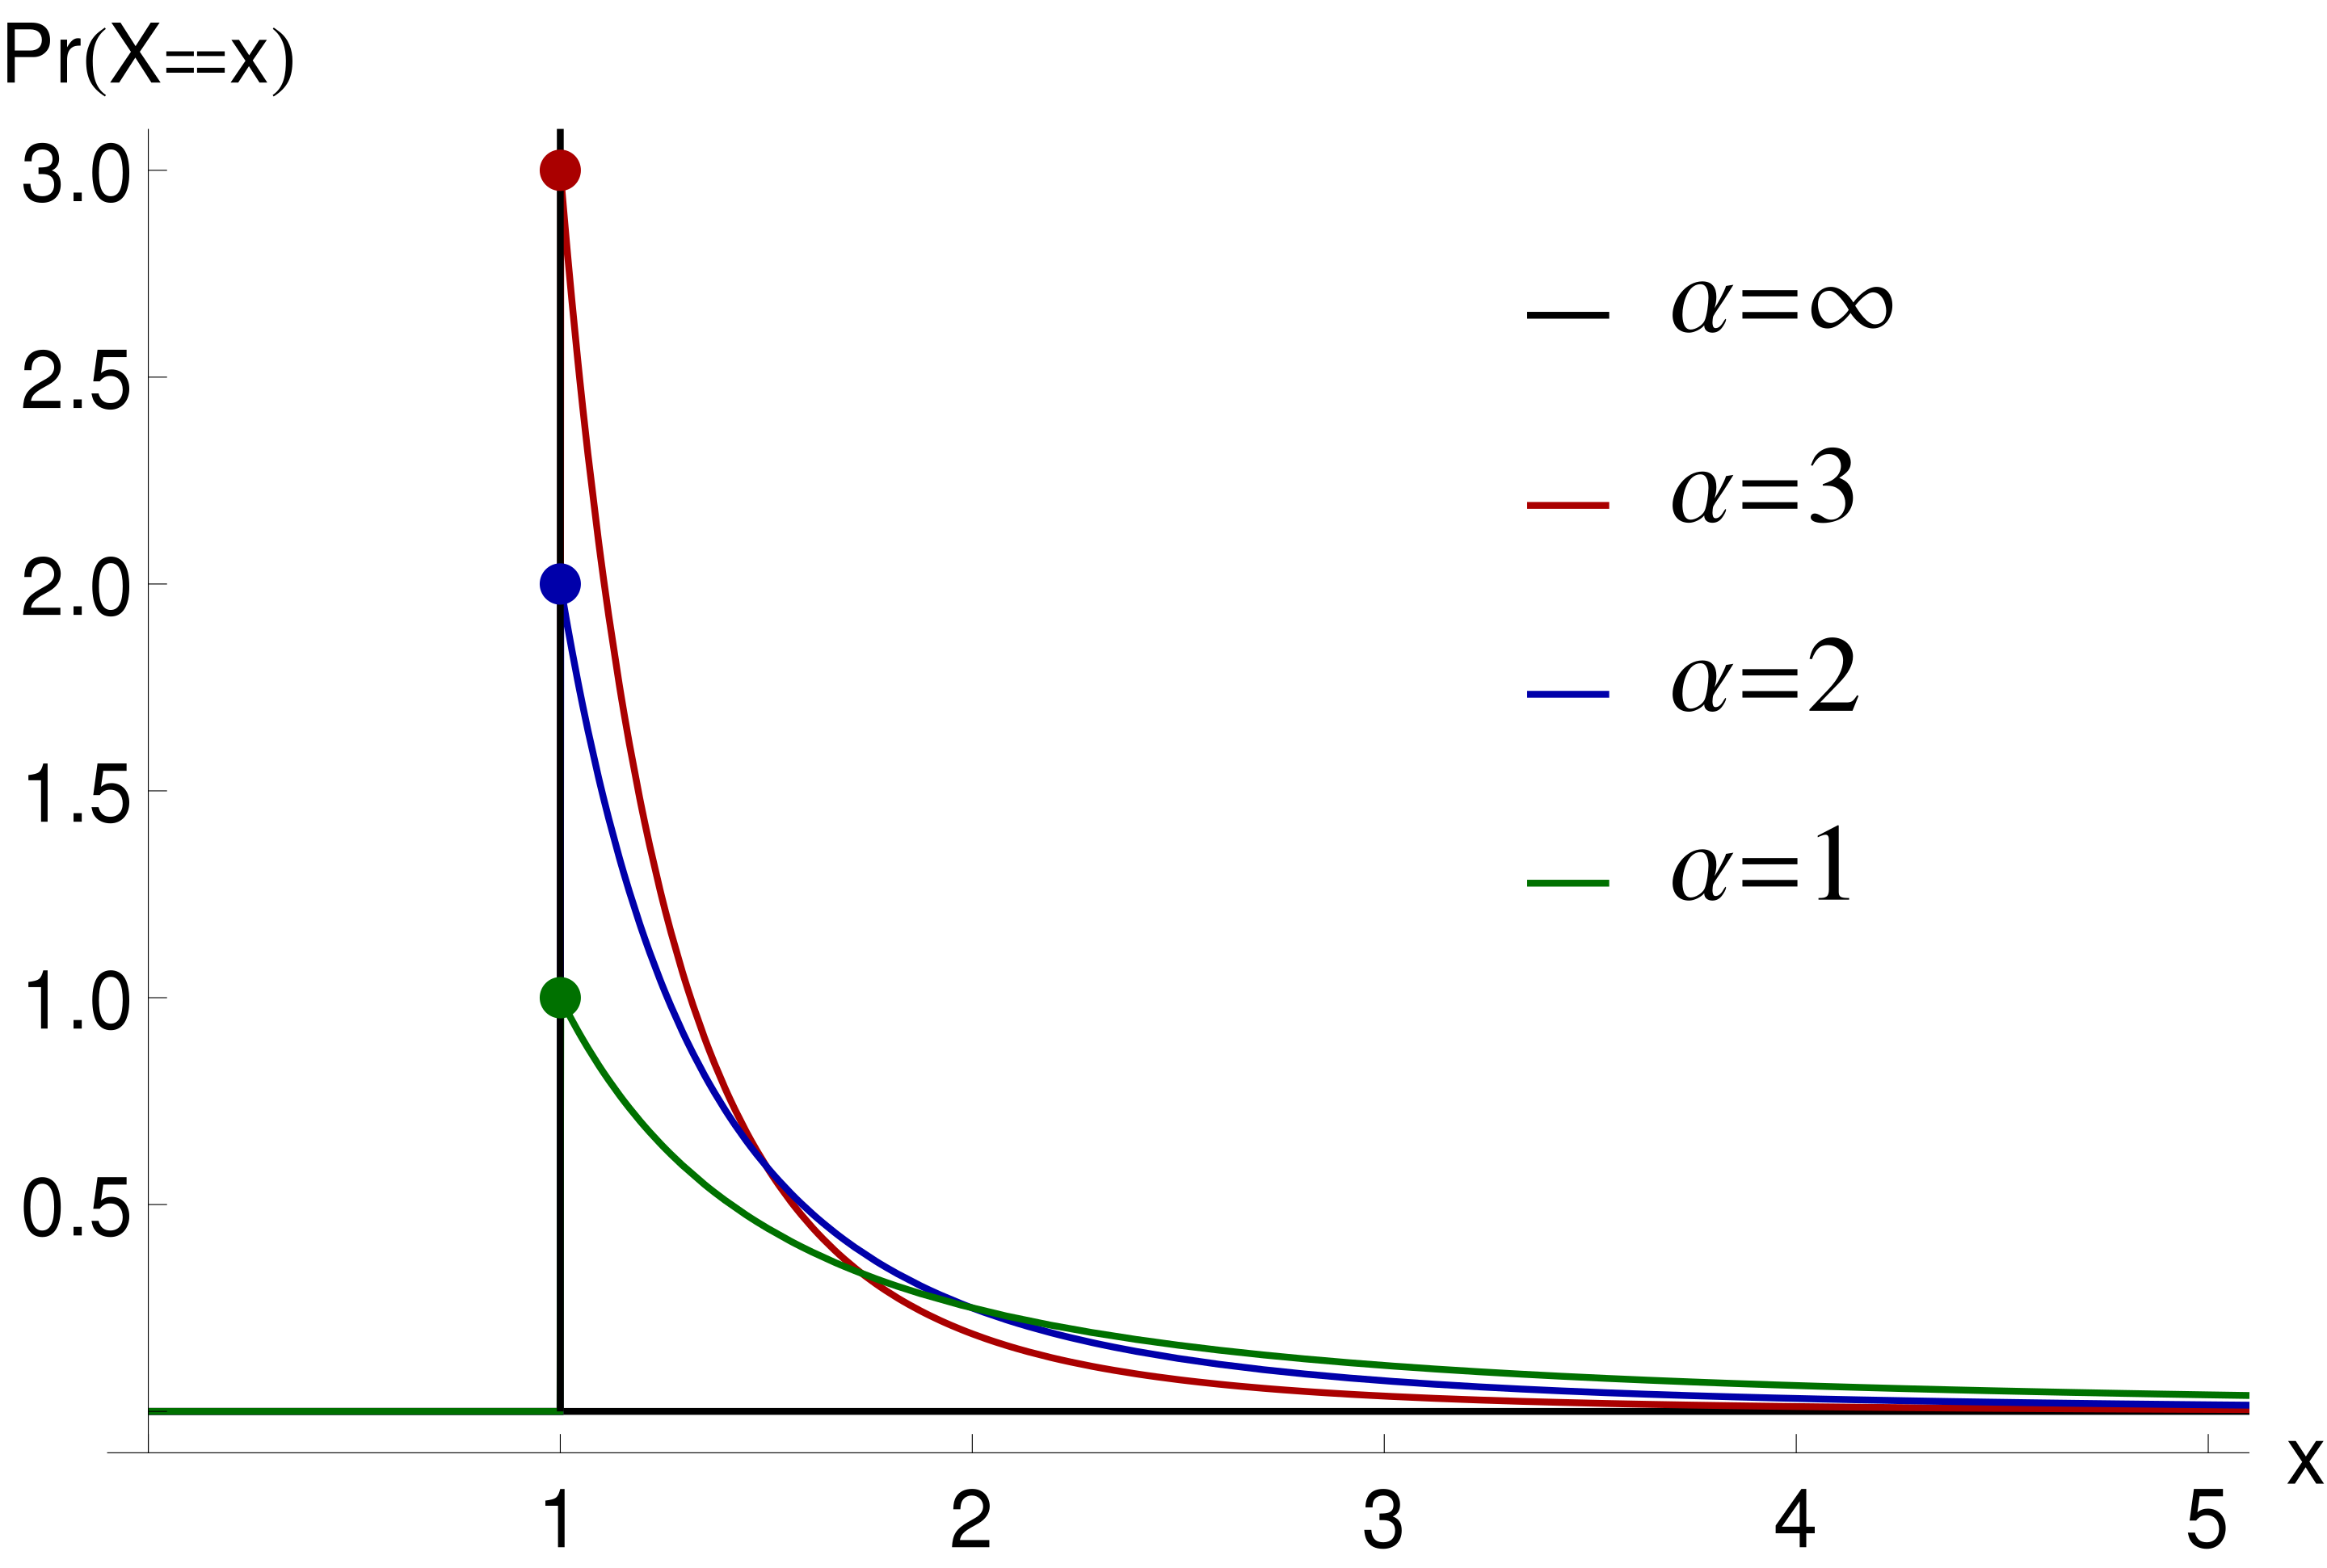
\includegraphics[width=0.4\columnwidth]{Probability_density_function_of_Pareto_distribution.png} ~~
  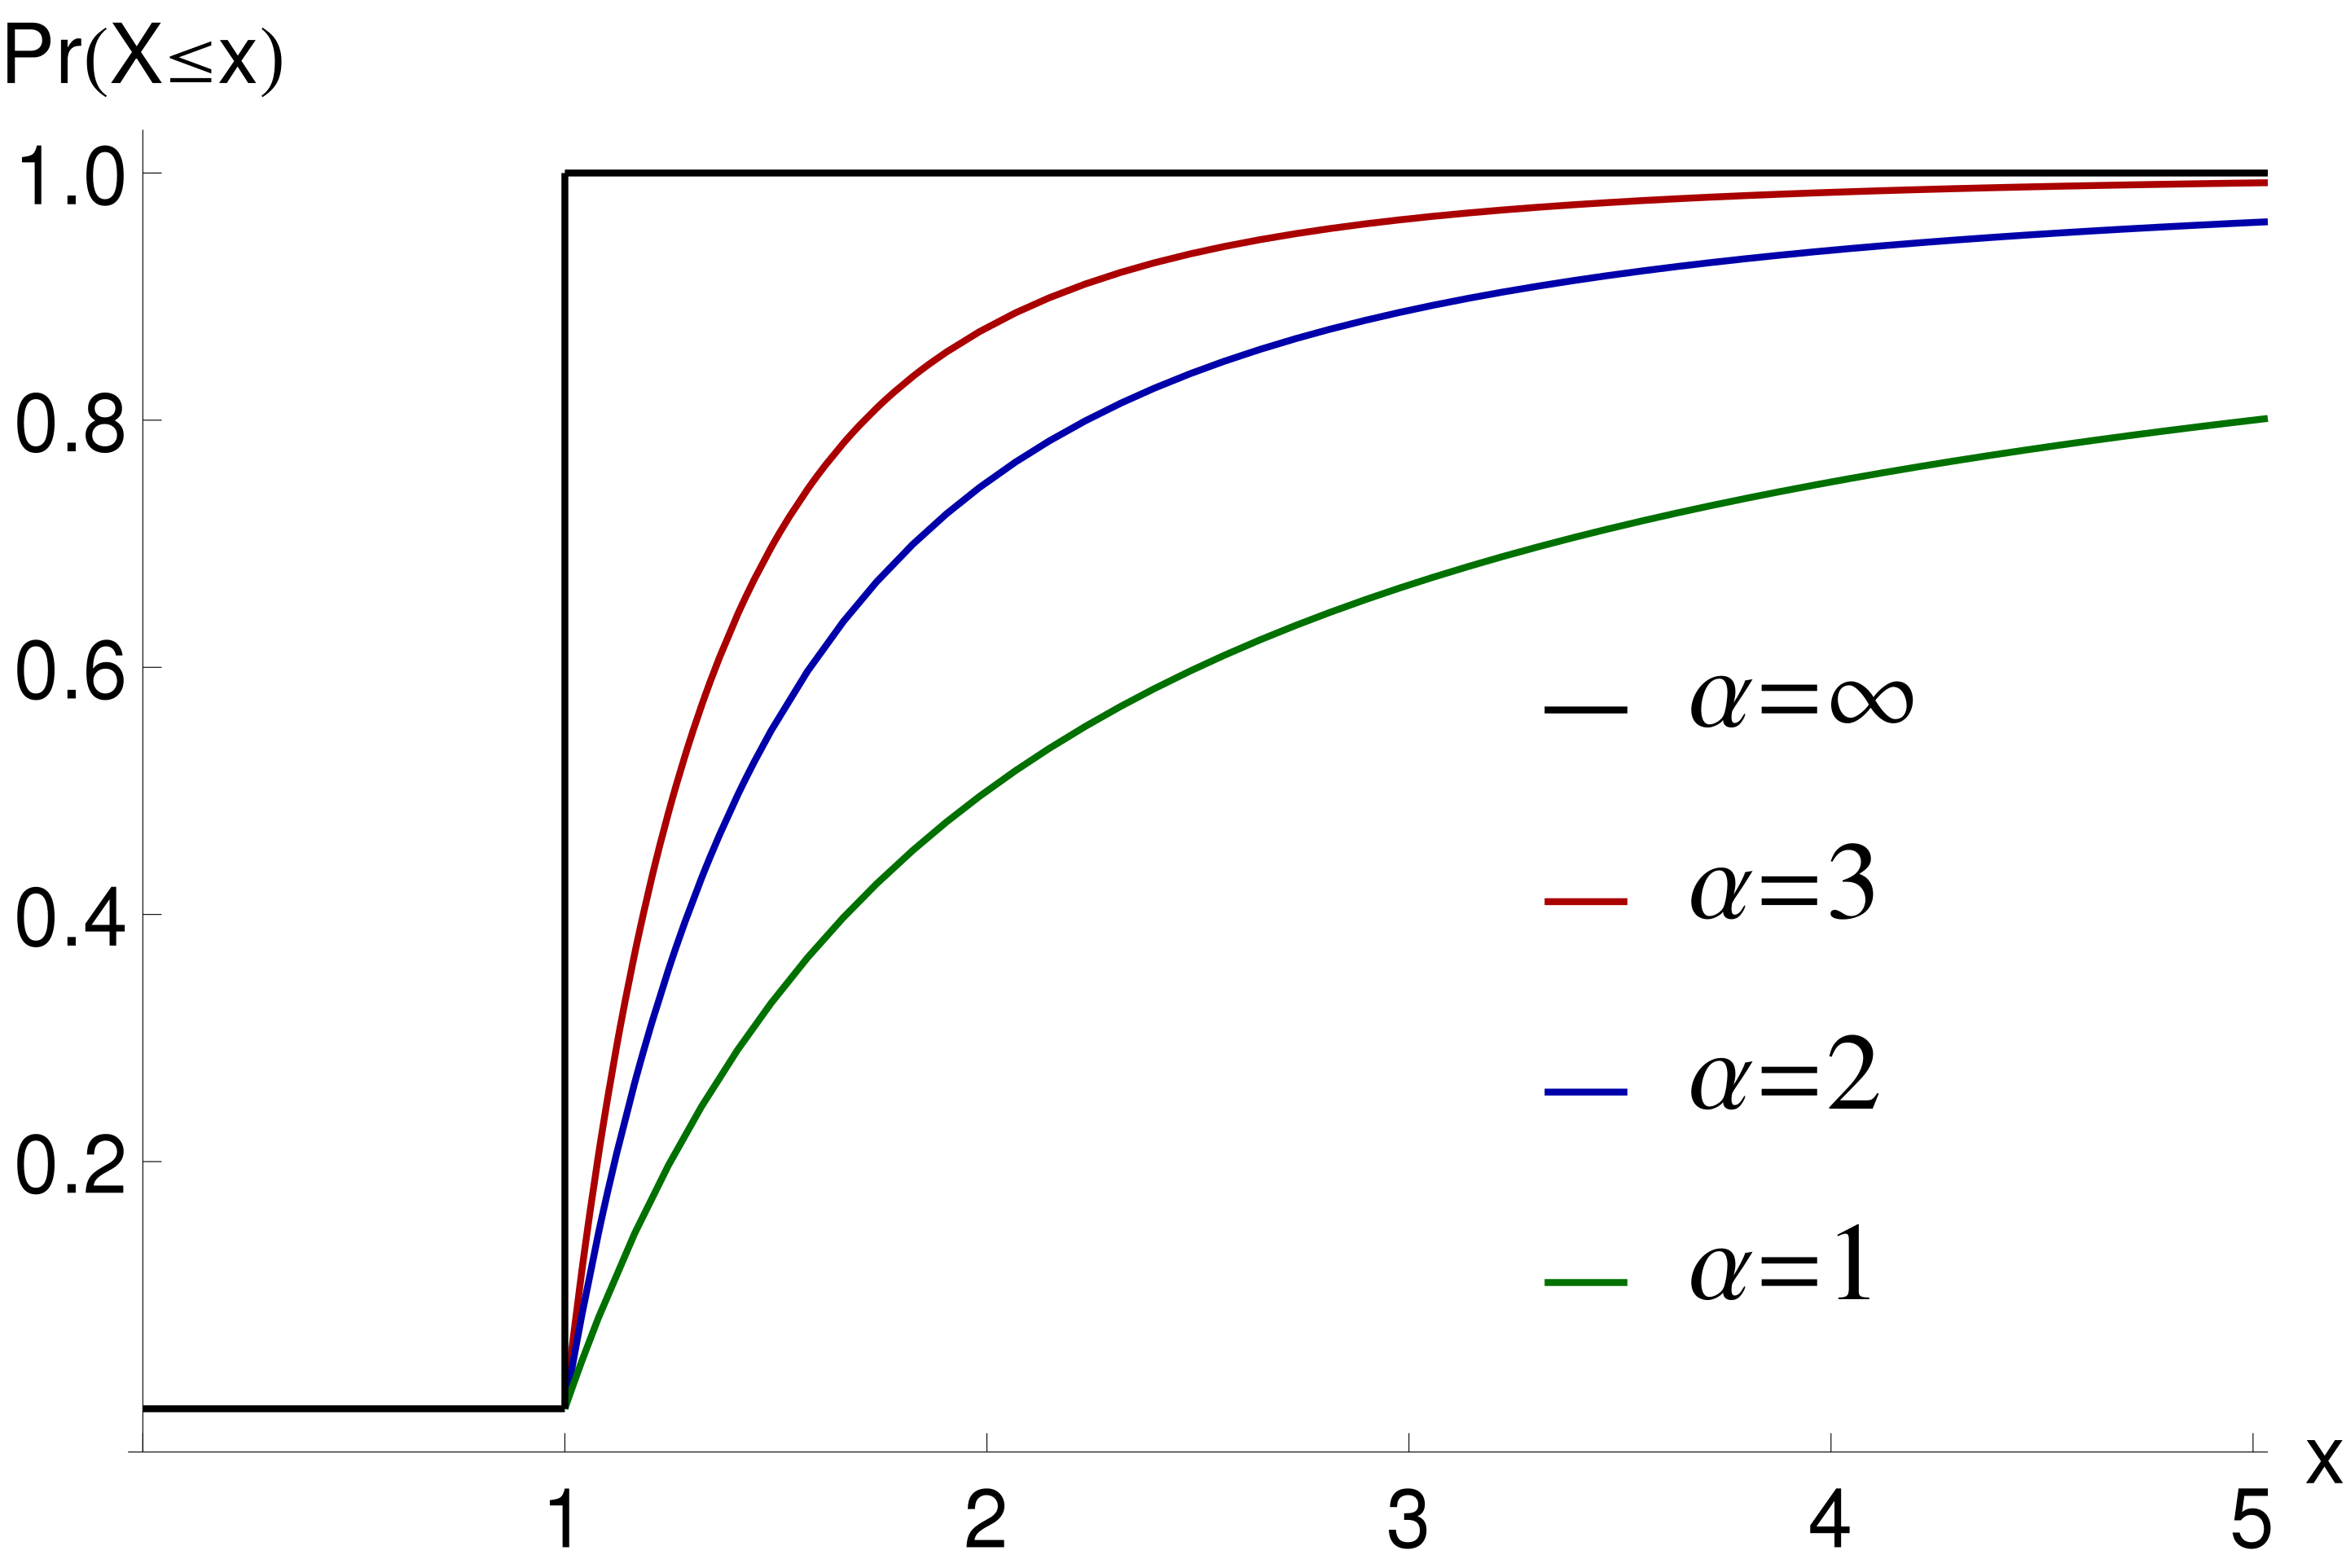
\includegraphics[width=0.4\columnwidth]{Cumulative_distribution_function_of_Pareto_distribution.png}
  \caption{Pareto Type I PDF's (left) \& CDF's (right) for various $\alpha$  with ${\displaystyle x_{\mathrm {m} }=1.}$}
\end{figure}
\end{center}

\hypertarget{a-probabilistic-model-of-the-testing-process}{%
\section{A probabilistic model of the testing
process}\label{a-probabilistic-model-of-the-testing-process}}

\hypertarget{model-parameters}{%
\subsection{Model parameters}\label{model-parameters}}

\bigskip

\begin{longtable}[]{@{}ll@{}}
\toprule
Parameter & Definition\tabularnewline
\midrule
\endhead
\(t\) & No.~of tests conducted\tabularnewline
\(n\) & No.~of cases detected\tabularnewline
\(\nu\) & True no. of cases (incl.~undetected)\tabularnewline
\(d = \frac{n}{\nu}\) & Fraction of cases detected\tabularnewline
\(p = \frac{n}{t}\) & Test positivity\tabularnewline
\(\tau = \frac{t}{\nu}\) & Testing coverage\tabularnewline
\(\tau_{min} := 1\) & Minimum testing coverage (Pareto distribution
parameter)\tabularnewline
\(\alpha\) & Testing efficiency coefficient (Pareto distribution
parameter)\tabularnewline
\bottomrule
\end{longtable}

\bigskip

\hypertarget{model-description}{%
\subsection{Model description}\label{model-description}}

\begin{itemize}
\item
  Consider all individuals in the testing-eligible population, arranged
  from high to low predicted infection probability (as determined by the
  applied testing strategy)
\item
  Assume testing proceeds from the invidiual with highest to the one
  with lowest predicted probility of infection.
\item
  Each detected case can be viewed as the final, successful attempt in a
  series of 1 or more testing attempts to find the next case.
\item
  The number of attempts required to find the next case can thus be
  modeled as a Pareto distribution, with most cases found after only few
  unsuccessful attempts, but a very large number of attempts being
  necessary to find all or almost all cases.
\item
  The Pareto cumulative distribution function describes the proportion
  of true cases that are detected given the number of tests performed
  per true case.
\item
  The testing efficiency coefficient \(\alpha\) describes how quickly
  the success rate (test prositivity) decreases with the number of tests
  per true case.
\item
  Model definition: the observed test positivity (proportion of positive
  tests within a time period and population) is related to the fraction
  of detected cases precisely as is the testing coverage (tests
  conducted per true case) to the CDF of a Pareto distribution. \#TODO
  say it better.
\end{itemize}

\hypertarget{model-derivation}{%
\subsection{Model derivation}\label{model-derivation}}

Define

\begin{equation}
F(\tau) = 1 - \left(\frac{\tau_{min}}{\tau} \right)^\alpha
\end{equation}

for \(\tau \ge \tau_{min}\), and \(F(\tau) = 0\) for
\(\tau < \tau_{min}\).

Setting \(\tau_{min} = 1\) and rewriting \(F\) as \(\frac{n}{\nu}\) this
yields

\begin{equation}
d = \frac{n}{\nu} = 1 - \left(\frac{\tau_{min}}{\tau}\right)^\alpha
\end{equation}

\[
\tau_{min} := 1
\]

\begin{equation}
d = \frac{n}{\nu} = 1 - \left( \frac{\nu}{} \right)
\end{equation}

\hypertarget{estimation-of-alpha}{%
\section{\texorpdfstring{Estimation of
\(\alpha\)}{Estimation of \textbackslash alpha}}\label{estimation-of-alpha}}

\begin{equation}
a = \int_a^b c(x)  dx 
\end{equation}

\textbf{data}
\url{https://www.ijidonline.com/article/S1201-9712(20)30444-6/fulltext\#secsect0095}

\begin{Shaded}
\begin{Highlighting}[]
\NormalTok{case\_data \textless{}{-}}\StringTok{ }\KeywordTok{read\_csv}\NormalTok{(}\StringTok{"data\_capture\_mark\_recapture.csv"}\NormalTok{) }\OperatorTok{\%\textgreater{}\%}
\StringTok{  }\KeywordTok{transmute}\NormalTok{(}
\NormalTok{    Country,}
    \DataTypeTok{Hidden\_cases =} \StringTok{\textasciigrave{}}\DataTypeTok{Hidden cases}\StringTok{\textasciigrave{}}\NormalTok{,}
    \DataTypeTok{Total\_cases =} \StringTok{\textasciigrave{}}\DataTypeTok{Total cases}\StringTok{\textasciigrave{}}\NormalTok{,}
    \DataTypeTok{Observed\_cases =} \StringTok{\textasciigrave{}}\DataTypeTok{Total\_cases}\StringTok{\textasciigrave{}} \OperatorTok{{-}}\StringTok{ }\NormalTok{Hidden\_cases}
\NormalTok{  )}
\end{Highlighting}
\end{Shaded}

\begin{verbatim}
## Parsed with column specification:
## cols(
##   Country = col_character(),
##   `Hidden cases` = col_number(),
##   `Total cases` = col_number(),
##   `95% CI` = col_character(),
##   `Total/observed` = col_double()
## )
\end{verbatim}

\begin{Shaded}
\begin{Highlighting}[]
\CommentTok{\#From our world in data}
\NormalTok{test\_data \textless{}{-}}\StringTok{ }\KeywordTok{read\_csv}\NormalTok{(}\StringTok{"covid{-}testing{-}all{-}observations.csv"}\NormalTok{) }\OperatorTok{\%\textgreater{}\%}
\StringTok{  }\KeywordTok{filter}\NormalTok{(}\KeywordTok{str\_detect}\NormalTok{(Entity, }\StringTok{"Italy|Germany|Spain|United Kingdom|Greece|Austria"}\NormalTok{)) }\OperatorTok{\%\textgreater{}\%}
\StringTok{  }\KeywordTok{filter}\NormalTok{(}\KeywordTok{str\_detect}\NormalTok{(Entity, }\StringTok{"tests performed|samples tested"}\NormalTok{)) }\OperatorTok{\%\textgreater{}\%}\StringTok{ }
\StringTok{  }\KeywordTok{mutate}\NormalTok{(}
    \DataTypeTok{Country =} \KeywordTok{case\_when}\NormalTok{(}
      \StringTok{\textasciigrave{}}\DataTypeTok{ISO code}\StringTok{\textasciigrave{}} \OperatorTok{==}\StringTok{ "AUT"} \OperatorTok{\textasciitilde{}}\StringTok{ "Austria"}\NormalTok{,}
      \StringTok{\textasciigrave{}}\DataTypeTok{ISO code}\StringTok{\textasciigrave{}} \OperatorTok{==}\StringTok{ "DEU"} \OperatorTok{\textasciitilde{}}\StringTok{ "Germany"}\NormalTok{,}
      \StringTok{\textasciigrave{}}\DataTypeTok{ISO code}\StringTok{\textasciigrave{}} \OperatorTok{==}\StringTok{ "GRC"} \OperatorTok{\textasciitilde{}}\StringTok{ "Greece"}\NormalTok{,}
      \StringTok{\textasciigrave{}}\DataTypeTok{ISO code}\StringTok{\textasciigrave{}} \OperatorTok{==}\StringTok{ "ITA"} \OperatorTok{\textasciitilde{}}\StringTok{ "Italy"}\NormalTok{,}
      \StringTok{\textasciigrave{}}\DataTypeTok{ISO code}\StringTok{\textasciigrave{}} \OperatorTok{==}\StringTok{ "ESP"} \OperatorTok{\textasciitilde{}}\StringTok{ "Spain"}\NormalTok{,}
      \StringTok{\textasciigrave{}}\DataTypeTok{ISO code}\StringTok{\textasciigrave{}} \OperatorTok{==}\StringTok{ "GBR"} \OperatorTok{\textasciitilde{}}\StringTok{ "UK"}\NormalTok{,}
      \OtherTok{TRUE} \OperatorTok{\textasciitilde{}}\StringTok{ }\OtherTok{NA\_character\_}
\NormalTok{    )}
\NormalTok{  ) }\OperatorTok{\%\textgreater{}\%}
\StringTok{  }\KeywordTok{filter}\NormalTok{(Date }\OperatorTok{==}\StringTok{ }\KeywordTok{as.Date}\NormalTok{(}\StringTok{"2020{-}04{-}17"}\NormalTok{)) }\OperatorTok{\%\textgreater{}\%}
\StringTok{  }\KeywordTok{select}\NormalTok{(}
\NormalTok{    Country,}
\NormalTok{    Date,}
    \DataTypeTok{Cumulative\_tests =} \StringTok{\textasciigrave{}}\DataTypeTok{Cumulative total}\StringTok{\textasciigrave{}}
\NormalTok{  ) }\OperatorTok{\%\textgreater{}\%}
\StringTok{  }\KeywordTok{filter}\NormalTok{(}\OperatorTok{!}\KeywordTok{is.na}\NormalTok{(Cumulative\_tests))}
\end{Highlighting}
\end{Shaded}

\begin{verbatim}
## Parsed with column specification:
## cols(
##   Entity = col_character(),
##   `ISO code` = col_character(),
##   Date = col_date(format = ""),
##   `Source URL` = col_character(),
##   `Source label` = col_character(),
##   Notes = col_character(),
##   `Cumulative total` = col_double(),
##   `Daily change in cumulative total` = col_double(),
##   `Cumulative total per thousand` = col_double(),
##   `Daily change in cumulative total per thousand` = col_double(),
##   `7-day smoothed daily change` = col_double(),
##   `7-day smoothed daily change per thousand` = col_double(),
##   `Short-term positive rate` = col_double(),
##   `Short-term tests per case` = col_double()
## )
\end{verbatim}

\begin{Shaded}
\begin{Highlighting}[]
\NormalTok{plotData \textless{}{-}}\StringTok{ }\NormalTok{case\_data }\OperatorTok{\%\textgreater{}\%}
\StringTok{  }\KeywordTok{inner\_join}\NormalTok{(test\_data, }\DataTypeTok{by =} \StringTok{"Country"}\NormalTok{) }\OperatorTok{\%\textgreater{}\%}
\StringTok{  }\KeywordTok{mutate}\NormalTok{(}
    \StringTok{\textasciigrave{}}\DataTypeTok{log(1{-}n/nu)}\StringTok{\textasciigrave{}}\NormalTok{ =}\StringTok{ }\KeywordTok{log}\NormalTok{(}\DecValTok{1}\OperatorTok{{-}}\NormalTok{(Observed\_cases}\OperatorTok{/}\NormalTok{Total\_cases)),}
    \StringTok{\textasciigrave{}}\DataTypeTok{log(nu/t)}\StringTok{\textasciigrave{}}\NormalTok{ =}\StringTok{ }\KeywordTok{log}\NormalTok{(Total\_cases}\OperatorTok{/}\NormalTok{Cumulative\_tests)}
\NormalTok{  )}
  


\NormalTok{mod.lm \textless{}{-}}\StringTok{ }\KeywordTok{lm}\NormalTok{(}\StringTok{\textasciigrave{}}\DataTypeTok{log(1{-}n/nu)}\StringTok{\textasciigrave{}} \OperatorTok{\textasciitilde{}}\StringTok{  }\DecValTok{{-}1} \OperatorTok{+}\StringTok{ \textasciigrave{}}\DataTypeTok{log(nu/t)}\StringTok{\textasciigrave{}}\NormalTok{, }\DataTypeTok{data =}\NormalTok{ plotData)}

\KeywordTok{ggplot}\NormalTok{(plotData, }\KeywordTok{aes}\NormalTok{(}\DataTypeTok{x =} \StringTok{\textasciigrave{}}\DataTypeTok{log(nu/t)}\StringTok{\textasciigrave{}}\NormalTok{, }\DataTypeTok{y =} \StringTok{\textasciigrave{}}\DataTypeTok{log(1{-}n/nu)}\StringTok{\textasciigrave{}}\NormalTok{,)) }\OperatorTok{+}
\StringTok{  }\KeywordTok{geom\_label}\NormalTok{(}\KeywordTok{aes}\NormalTok{(}\DataTypeTok{label =}\NormalTok{ Country), }\DataTypeTok{nudge\_y =} \FloatTok{0.1}\NormalTok{) }\OperatorTok{+}
\StringTok{  }\KeywordTok{geom\_point}\NormalTok{() }\OperatorTok{+}
\StringTok{  }\CommentTok{\#geom\_smooth(method=\textquotesingle{}lm\textquotesingle{}, formula= y \textasciitilde{}  {-}1 + x)}
\StringTok{  }\KeywordTok{geom\_abline}\NormalTok{(}\DataTypeTok{slope =} \KeywordTok{coef}\NormalTok{(mod.lm), }\DataTypeTok{intercept =}\DecValTok{0}\NormalTok{) }\OperatorTok{+}
\StringTok{  }\KeywordTok{coord\_cartesian}\NormalTok{(}\DataTypeTok{xlim =} \KeywordTok{c}\NormalTok{(}\OperatorTok{{-}}\DecValTok{3}\NormalTok{, }\DecValTok{0}\NormalTok{), }\DataTypeTok{ylim =} \KeywordTok{c}\NormalTok{(}\OperatorTok{{-}}\DecValTok{1}\NormalTok{, }\DecValTok{0}\NormalTok{))}
\end{Highlighting}
\end{Shaded}

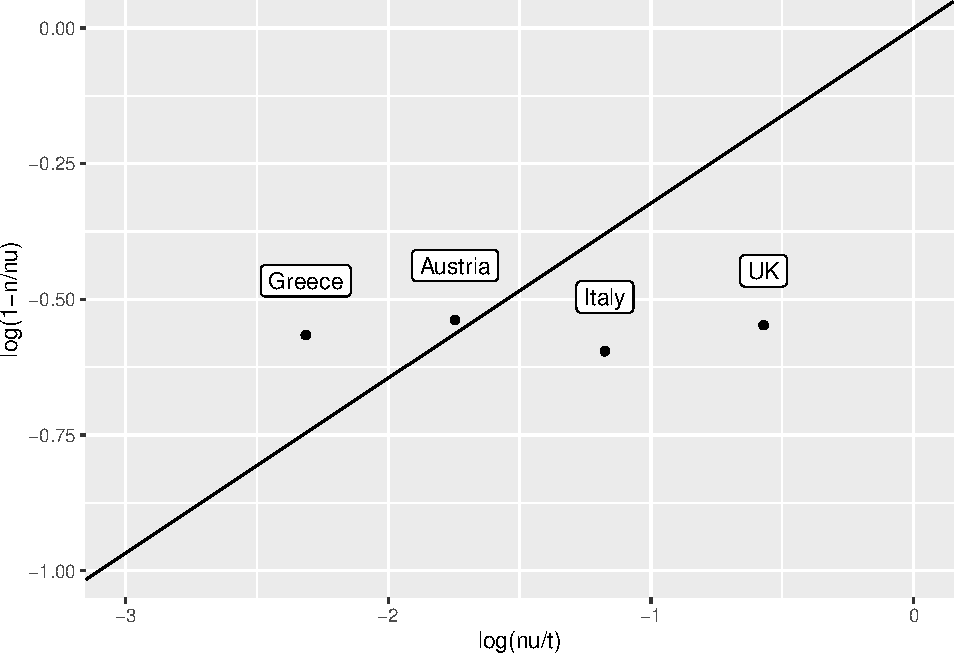
\includegraphics{pareto_model_of_testing_files/figure-latex/unnamed-chunk-2-1.pdf}

\begin{Shaded}
\begin{Highlighting}[]
\NormalTok{pander}\OperatorTok{::}\KeywordTok{pander}\NormalTok{(mod.lm)}
\end{Highlighting}
\end{Shaded}

\begin{longtable}[]{@{}ccccc@{}}
\caption{Fitting linear model: \texttt{log(1-n/nu)} \textasciitilde{} -1
+ \texttt{log(nu/t)}}\tabularnewline
\toprule
\begin{minipage}[b]{0.21\columnwidth}\centering
~\strut
\end{minipage} & \begin{minipage}[b]{0.13\columnwidth}\centering
Estimate\strut
\end{minipage} & \begin{minipage}[b]{0.16\columnwidth}\centering
Std. Error\strut
\end{minipage} & \begin{minipage}[b]{0.12\columnwidth}\centering
t value\strut
\end{minipage} & \begin{minipage}[b]{0.13\columnwidth}\centering
Pr(\textgreater\textbar t\textbar)\strut
\end{minipage}\tabularnewline
\midrule
\endfirsthead
\toprule
\begin{minipage}[b]{0.21\columnwidth}\centering
~\strut
\end{minipage} & \begin{minipage}[b]{0.13\columnwidth}\centering
Estimate\strut
\end{minipage} & \begin{minipage}[b]{0.16\columnwidth}\centering
Std. Error\strut
\end{minipage} & \begin{minipage}[b]{0.12\columnwidth}\centering
t value\strut
\end{minipage} & \begin{minipage}[b]{0.13\columnwidth}\centering
Pr(\textgreater\textbar t\textbar)\strut
\end{minipage}\tabularnewline
\midrule
\endhead
\begin{minipage}[t]{0.21\columnwidth}\centering
\textbf{\texttt{log(nu/t)}}\strut
\end{minipage} & \begin{minipage}[t]{0.13\columnwidth}\centering
0.3226\strut
\end{minipage} & \begin{minipage}[t]{0.16\columnwidth}\centering
0.08363\strut
\end{minipage} & \begin{minipage}[t]{0.12\columnwidth}\centering
3.858\strut
\end{minipage} & \begin{minipage}[t]{0.13\columnwidth}\centering
0.03078\strut
\end{minipage}\tabularnewline
\bottomrule
\end{longtable}

\begin{Shaded}
\begin{Highlighting}[]
\NormalTok{alpha \textless{}{-}}\StringTok{ }\KeywordTok{coef}\NormalTok{(mod.lm) }\OperatorTok{\%\textgreater{}\%}\StringTok{ }\NormalTok{as.numeric}
\end{Highlighting}
\end{Shaded}

\begin{Shaded}
\begin{Highlighting}[]
\NormalTok{one\_step\_d \textless{}{-}}\StringTok{ }\ControlFlowTok{function}\NormalTok{(nu, t, alpha)\{}
  \DecValTok{1}\OperatorTok{{-}}\NormalTok{(nu}\OperatorTok{/}\NormalTok{t)}\OperatorTok{\^{}}\NormalTok{alpha}
\NormalTok{\}}

\NormalTok{calc\_d \textless{}{-}}\StringTok{ }\KeywordTok{Vectorize}\NormalTok{(}\ControlFlowTok{function}\NormalTok{(n, t, alpha)\{}
\NormalTok{  d \textless{}{-}}\StringTok{ }\FloatTok{0.5} \CommentTok{\#starting value}
  \ControlFlowTok{for}\NormalTok{(i }\ControlFlowTok{in} \DecValTok{1}\OperatorTok{:}\DecValTok{1000}\NormalTok{) \{}
\NormalTok{    new\_d \textless{}{-}}\StringTok{ }\KeywordTok{one\_step\_d}\NormalTok{(}\DataTypeTok{nu =}\NormalTok{ n}\OperatorTok{*}\NormalTok{d, }\DataTypeTok{t =}\NormalTok{ t, alpha)}
    \ControlFlowTok{if}\NormalTok{(new\_d }\OperatorTok{==}\StringTok{ }\NormalTok{d) \{}
      \ControlFlowTok{break}
\NormalTok{    \} }\ControlFlowTok{else}\NormalTok{ \{}
\NormalTok{        d \textless{}{-}}\StringTok{ }\NormalTok{new\_d}
\NormalTok{      \}}
\NormalTok{  \}}
\NormalTok{  d}
\NormalTok{\})}

\KeywordTok{calc\_d}\NormalTok{(}\DataTypeTok{n =} \DecValTok{172433}\NormalTok{, }\DataTypeTok{t =} \DecValTok{1244108}\NormalTok{, alpha)}
\end{Highlighting}
\end{Shaded}

\begin{verbatim}
## [1] 0.5612721
\end{verbatim}

\hypertarget{estimating-the-detected-proportion-d-from-data-given-alpha}{%
\section{\texorpdfstring{Estimating the detected proportion d from data,
given
\(\alpha\)}{Estimating the detected proportion d from data, given \textbackslash alpha}}\label{estimating-the-detected-proportion-d-from-data-given-alpha}}

\begin{Shaded}
\begin{Highlighting}[]
\NormalTok{plotData \textless{}{-}}\StringTok{ }\KeywordTok{tibble}\NormalTok{(}
  \DataTypeTok{tau =} \DecValTok{1}\OperatorTok{:}\DecValTok{1000}
\NormalTok{) }\OperatorTok{\%\textgreater{}\%}
\KeywordTok{mutate}\NormalTok{(}
  \DataTypeTok{d =} \KeywordTok{calc\_d}\NormalTok{(}\DataTypeTok{n =} \DecValTok{100}\NormalTok{, }\DataTypeTok{t =}\NormalTok{ tau}\OperatorTok{*}\DecValTok{100}\NormalTok{, }\DataTypeTok{alpha =}\NormalTok{ alpha )    }
\NormalTok{)}

\KeywordTok{ggplot}\NormalTok{(plotData, }\KeywordTok{aes}\NormalTok{(}\DataTypeTok{x =}\NormalTok{ tau, }\DataTypeTok{y =}\NormalTok{ d)) }\OperatorTok{+}
\StringTok{  }\KeywordTok{geom\_line}\NormalTok{() }\OperatorTok{+}
\StringTok{  }\KeywordTok{scale\_x\_log10}\NormalTok{() }\OperatorTok{+}
\StringTok{  }\KeywordTok{theme\_minimal}\NormalTok{()}
\end{Highlighting}
\end{Shaded}

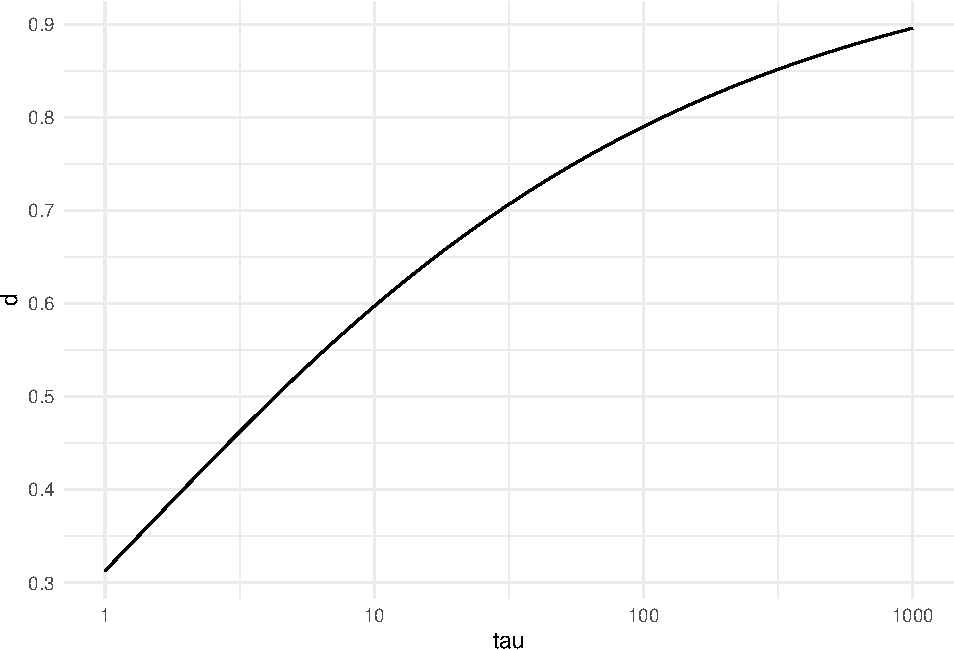
\includegraphics{pareto_model_of_testing_files/figure-latex/unnamed-chunk-4-1.pdf}

\hypertarget{the-transmission-reducing-effect-of-testing-and-contact-tracing}{%
\section{The transmission-reducing effect of testing and contact
tracing}\label{the-transmission-reducing-effect-of-testing-and-contact-tracing}}

..

\end{document}
